\documentclass[
  digital, %% The `digital` option enables the default options for the
           %% digital version of a document. Replace with `printed`
           %% to enable the default options for the printed version
           %% of a document.
  color,   %% Uncomment these lines (by removing the %% at the
           %% beginning) to use color in the digital version of your
           %% document
  table,   %% The `table` option causes the coloring of tables.
           %% Replace with `notable` to restore plain LaTeX tables.
  twoside, %% The `twoside` option enables double-sided typesetting.
           %% Use at least 120 g/m² paper to prevent show-through.
           %% Replace with `oneside` to use one-sided typesetting;
           %% use only if you don’t have access to a double-sided
           %% printer, or if one-sided typesetting is a formal
           %% requirement at your faculty.
  nolof,   %% The `lof` option prints the List of Figures. Replace
           %% with `nolof` to hide the List of Figures.
  nolot,   %% The `lot` option prints the List of Tables. Replace
           %% with `nolot` to hide the List of Tables.
  %% More options are listed in the user guide at
  %% <http://mirrors.ctan.org/macros/latex/contrib/fithesis/guide/mu/fi.pdf>.
]{fithesis3}
%% The following section sets up the locales used in the thesis.
\usepackage[resetfonts]{cmap} %% We need to load the T2A font encoding
\usepackage[T1,T2A]{fontenc}  %% to use the Cyrillic fonts with Russian texts.
\usepackage[
  main=czech,   %% By using `czech` or `slovak` as the main locale
                %% instead of `english`, you can typeset the thesis
                %% in either Czech or Slovak, respectively.
  english, german, russian, czech, slovak %% The additional keys allow
]{babel}        %% foreign texts to be typeset as follows:
%%
%%   \begin{otherlanguage}{german}  ... \end{otherlanguage}
%%   \begin{otherlanguage}{russian} ... \end{otherlanguage}
%%   \begin{otherlanguage}{czech}   ... \end{otherlanguage}
%%   \begin{otherlanguage}{slovak}  ... \end{otherlanguage}
%%
%% For non-Latin scripts, it may be necessary to load additional
%% fonts:
\usepackage{paratype}
\def\textrussian#1{{\usefont{T2A}{PTSerif-TLF}{m}{rm}#1}}
%%
%% The following section sets up the metadata of the thesis.
\thesissetup{
    date        = \the\year/\the\month/\the\day,
    university  = mu,
    faculty     = fi,
    type        = bc,
    author      = Dominik Salvet,
    gender      = m,
    advisor     = {prof. Ing. Václav Přenosil, CSc.},
    title       = {Návrh modelu procesoru},
    TeXtitle    = {Návrh modelu procesoru},
    titleEn     = {Design of the Processor Model},
    TeXtitleEn  = {Design of the Processor Model},
    keywords    = {procesor, RISC, ISA, pipeline, VHDL, ALU, testbench, přerušení},
    TeXkeywords = {procesor, RISC, ISA, pipeline, VHDL, ALU, testbench, přerušení},
    keywordsEn  = {processor, RISC, ISA, pipeline, VHDL, ALU, testbench, interrupt},
    TeXkeywordsEn = {processor, RISC, ISA, pipeline, VHDL, ALU, testbench, interrupt},
    abstract    = {%
      Cílem této práce je navrhnout model 64bitového procesoru vlastní instrukční sady a doložit jeho funkčnost. Tato instrukční sada respektuje RISC principy při snaze zvýšit hustotu výsledného kódu. Za tímto účelem definuje výhradně instrukční slova s délkou 16 bitů.
      
      Referenční model implementující tuto instrukční sadu je popsán v~jazyce VHDL pomocí základního pětistupňového pipeliningu. Lze ho simulovat pomocí programu GHDL a, s malým úsilím, implementovat do hradlového pole dostatečné kapacity. Správné chování procesoru a~jeho stěžejních modulů je doloženo pomocí test bench souborů.
    },
    abstractEn  = {%
      The goal of this work is to design a 64-bit processor model of a custom instruction set architecture and verify its operation. The instruction set respects RISC principles while putting effort into decreasing final code density. For this purpose, it defines 16-bit instruction words only.
      
      The reference model, which implements this instruction set, is described in VHDL language using basic five-stage pipelining. It may be simulated using GHLD software and, with little effort, implemented into gate array of sufficient capacity. The correct behavior of the processor and its key modules is verified by test bench files.
    },
    thanks      = {%
      Tímto bych chtěl vyjádřit velké poděkování vedoucímu mé bakalářské práce prof. Ing. Václavu Přenosilovi, CSc. za cenné rady nejen v~rozsahu této práce. Zvláště bych chtěl poděkovat za projevenou trpělivost, čehož si velmi vážím.
      
      Děkuji také mé rodině za neustálou podporu a důvěru.
    },
    bib         = example.bib,
    %% Uncomment the following line (by removing the %% at the
    %% beginning) and replace `assignment.pdf` with the filename
    %% of your scanned thesis assignment.
%%    assignment         = assignment.pdf,
}
\usepackage{makeidx}      %% The `makeidx` package contains
\makeindex                %% helper commands for index typesetting.
%% These additional packages are used within the document:
\usepackage{paralist} %% Compact list environments
\usepackage{amsmath}  %% Mathematics
\usepackage{amsthm}
\usepackage{amsfonts}
\usepackage{url}      %% Hyperlinks
\usepackage{tabularx} %% Tables
\usepackage{tabu}
\usepackage{booktabs}
\usepackage{listings} %% Source code highlighting
\lstset{
  basicstyle      = \ttfamily,
  identifierstyle = \color{black},
  keywordstyle    = \color{blue},
  keywordstyle    = {[2]\color{cyan}},
  keywordstyle    = {[3]\color{olive}},
  stringstyle     = \color{teal},
  commentstyle    = \itshape\color{magenta},
  breaklines      = true,
}
\usepackage{floatrow} %% Putting captions above tables
\usepackage{dirtree}
\floatsetup[table]{capposition=top}
\begin{document}
\chapter*{Úvod}
\addcontentsline{toc}{chapter}{Úvod}
Návrh procesoru je obecně velmi rozsáhlá činnost několika vědních oborů vyžadující pokročilé znalosti číslicové techniky, hardwarových principů, principů nízkoúrovňového softwaru i specifických oblastí fyziky. Návrh modelu procesoru je podmnožinou této činnosti a omezuje se pouze na návrh logické struktury procesoru, příp. i tvorby jeho virtuální implementace.

Tato práce představuje model 64bitového RISC\footnote{Reduced Instruction Set Computer -- počítač s redukovanou instrukční sadou} procesoru vlastní architektury a popisuje jeho funkce. K vytvoření takového modelu je nejdříve definována vlastní architektura instrukční sady (dále jen ISA\footnote{Z anglického překladu Instruction Set Architecture}), která používá menší šířku instrukčního slova, než je běžné u~architektur s podobnými rysy. To zpravidla vede k nižším paměťovým nárokům většiny programů, což se nakonec může pozitivně projevit i ve výkonu procesoru \parencite{bunda93}. Tímto přístupem se totiž snižuje tlak na instrukční paměť, která je v moderních procesorech\footnote{Moderním procesorem rozumíme procesor pro osobní počítače.} implementována jako instrukční cache a významně se podílí na celkovém výkonu procesoru. Hlavní motivací práce je tedy prozkoumat dopad menších instrukcí na samotný návrh modelu procesoru (dále už jen procesor) a jeho architekturu.

Součástí práce je i referenční mikroarchitektura, která zmíněnou ISA kompletně implementuje. Je popsána v jazyce VHDL metodou pětistupňového pipeliningu a podporuje i okamžitá přerušení. Hlavní modul procesoru vystavuje jednoduché rozhraní pro komunikaci s~instrukční a datovou pamětí. Pakliže jsou tyto paměťové moduly dostupné, je procesor připraven na umístění do hradlového pole a~demonstraci jeho možností na skutečném hardwaru.

V neposlední řadě je práce doprovázena i test bench soubory, které ověřují funkčnost procesoru i jeho klíčových komponent. K simulaci procesoru na počítači se používá open-source program GHDL\footnote{G Hardware Design Language -- G jazyk pro návrh hardwaru} a~pro snadnější práci s celým build systémem procesoru byl vytvořen i~jednoduchý \texttt{makefile}.

Samotný text práce je rozčleněn do několika dílčích kapitol. První kapitola se zabývá ustanovením základních vlastností ISA. Na základě definic z první kapitoly se druhá kapitola zabývá návrhem ISA a zmiňuje i významné procesorové architektury, které měly vliv na její vývoj. Ve třetí kapitole je tato navržená ISA implementována popisem v jazyce VHDL. Zahrnuje i detailní vhled do mikroarchitektury procesoru. Praktičtější povahu má kapitola čtvrtá, která ukazuje, jak obsluhovat build systém procesoru. Důraz je kladen zejména na simulaci procesoru pro účely testování.

Model procesoru vzniknuvší v rámci této práce nese označení RISC63 a jeho zdrojové kódy a ostatní materiály jsou veřejně dostupné z GitHub repositáře\footnote{\url{https://github.com/dominiksalvet/risc63}} pod Apache 2.0 licencí.

\chapter{Vlastnosti instrukční sady}
Instrukční sada je abstraktní soubor pravidel, který jednoznačně definuje rozsah funkcionality procesoru. Definuje tedy jednotlivé strojové instrukce a jejich sémantiku, architekturální registry, organizaci paměti, mechanismus přerušení a další. Tyto vlastnosti mají přímý vliv na výslednou implementaci procesoru. Pro programátora, resp. kompilátor, se pak jedná o dostupné prostředky procesoru implementujícího danou ISA.

V této kapitole jsou popsány významné vlastnosti ISA v kontextu této práce. Asi nejznámější vlastností ISA je její typ. Ačkoliv přesná definice tohoto pojmu neexistuje, je široce užíván ve snaze implicitně vystihnout dílčí vlastnosti ISA. Další zkoumané vlastnosti ISA pak zahrnují bitovou šířku dat, bitovou šířku instrukcí, architekturální registry, třídu instrukční sady a organizaci paměti. Na základě těchto definic jsme pak schopni v další kapitole odvodit možné dostupné instrukce ISA a jejich vlastnosti.

Každá podkapitola se věnuje pouze jedné z uvedených vlastností. Popíše danou vlastnost, jak se obvykle volí její parametry, možný dopad na architekturu procesoru a uvede i soudobé populární hodnoty parametrů (rok 2020).

\section{Typ instrukční sady}
Typem instrukční sady rozumíme pro účely této práce klasifikaci podle složitosti procesorové architektury. Přestože se nejedná o žádný přesně definovaný postup, je daná ISA podle převažujících rysů zařazena do nejvhodnějšího, zpravidla již existujícího, typu ISA. Velmi vzácně se však může stát, že nová ISA je natolik specifická, aby dala vzniknout novému typu ISA, který ji vystihuje \parencite{burger04}.

Pro potřeby této práce se v níže uvedené analýze omezíme jen na dva nejrozšířenější typy ISA, kterými jsou CISC\footnote{Complex Instruction Set Computer -- počítač s komplexní instrukční sadou} a RISC.

\subsection{CISC}
CISC lze považovat za nejstarší ustanovený typ ISA. Nejvíce jej zviditelnila firma Intel se svou CISC architekturou x86, která byla později nahrazena kompatibilní CISC architekturou AMD64. CISC se vyznačuje především obsáhlým repertoárem instrukcí. Obecně také definuje proměnlivou délku těchto instrukcí, nižší počet pracovních registrů a~více podporovaných adresních módů pro přístup k paměti.

Lze konstatovat, že tento typ ISA je na ústupu, protože její výhody spojené s nízkými paměťovými nároky programů již nejsou tak důležité, jako tomu bylo dříve. Navíc dekodér CISC instrukcí v celé řadě případů limituje efektivní implementaci moderních mechanismů pro zvýšení výkonu procesoru. Toto tvrzení podporuje i skutečnost, že x86/AMD64 je nyní jedinou rozšířenou CISC architekturou.

\subsection{RISC}
Vznik RISC architektury lze připsat snaze zvýšit výkon tehdejších CISC procesorů, které byly poměrně složité. Zároveň se tehdy snižovala cena operační paměti. Tyto okolnosti vyústily v ustanovení nového typu ISA, jehož hlavním pilířem je jednoduchost výsledné mikroarchitektury. Z toho důvodu RISC procesory obsahují jen jednoduché a nejpoužívanější instrukce, mají vyšší počet pracovních registrů (obecného použití) a podporují pouze několik adresních módu.

Jednodušší RISC architektury definují instrukce s pevnou délkou. Pokročilejší RISC architektury většinou definují vedle toho i kratší instrukce, označovány jako komprimované, které mohou představovat aliasy pro nejpoužívanější instrukce plné velikosti~\mbox{\parencite[97--113]{waterman19}}. Motivací k tomuto přístupu je zvýšit hustotu kódu, což vede ke snížení tlaku na instrukční cache, a~to pak zvyšuje výkon procesoru.

Dnešní RISC architektury dosahují hustoty kódu, která je srovnatelná nebo dokonce lepší než hustota kódu CISC architektur \parencite{waterman15}. Stále přitom nabízí výhody spojené s jednoduchostí RISC návrhu. Obecně se pak dá tvrdit, že přízeň k RISC architekturám roste od doby jejich vzniku. Mnoho aktuálních a dokonce i nově vznikajících architektur je právě typu RISC.\footnote{Viz např. \url{https://riscv.org}.}

\section{Bitová šířka dat}
Bitová šířka dat, též označovaná jako bitová šířka slova, představuje největší počet bitů dat, se kterými dokáže ISA nativně pracovat. Při práci s daty vyšší bitové šířky je zapotřebí implementovat požadovanou operaci pomocí několika dílčích kroků.

Hodnota bitové šířky dat má klíčový význam pro mnoho vlastností procesoru. Přímo ovlivňuje bitovou šířku aritmeticko-logické jednotky (dále jen ALU\footnote{Z anglického překladu Arithmetic Logic Unit}) a pracovních registrů. Velmi často pak ovlivňuje i~architekturu jiných modulů procesoru a bitové šířky sběrnic, se kterými procesor pracuje. Může se jednat o architekturu cache a bitové šířky datové\footnote{Tato sběrnice často udává konečnou bitovou šířku přenosu dat.} i adresní sběrnice procesoru.

Menší hodnoty bitové šířky dat obecně znamenají rychlejší propagaci dat skrze procesor a nižší požadavky na hardwarové prostředky. Větší hodnoty bitové šířky dat ovšem umožňují procesoru efektivněji pracovat s daty vyšších bitových šířek a adresovat větší paměťový prostor. Volba bitové šířky dat se zejména odvozuje z potřebné kapacity paměťového prostoru, který má být schopen procesor efektivně adresovat. Zvýšit kapacitu adresovatelného paměťového prostoru již existující procesorové architektury bývá totiž netriviální úkon.

Nejčastější šířka dat v moderních procesorech je 64 bitů a zřídka se ještě používají procesory s šířkou dat 32 bitů. Takové procesory jsou souhrnně označovány jako 64bitové, resp. 32bitové. Důvodem vzestupu popularity 64bitové šířky dat byly zejména zvyšující se paměťové požadavky softwaru a s tím spjatá potřeba navýšení kapacity paměťového prostoru adresovatelného procesorem. Tento trend byl doprovázen také postupnou transformací 32bitového softwaru na 64bitový, který je schopen možností 64bitového procesoru využít.

\section{Bitová šířka instrukcí}
Bitová šířka instrukcí, též označovaná jako bitová délka instrukčního slova, představuje počet bitů instrukčního slova dané ISA. Tento pojem však není široce zavedený, protože existují architektury, které mají proměnlivou délku instrukce. Jednoznačně jej lze tedy aplikovat jen na architektury s pevnou délkou instrukcí. Z hodnoty bitové šířky instrukcí lze přímo odvodit celkový počet unikátních instrukcí vykonatelných procesorem.

Při volbě hodnoty bitové šířky instrukcí je nutné si uvědomit, že~mnoho instrukcí bude obsahovat bity reprezentující indexy pro pracovní registry procesoru nebo bity reprezentující konstanty. A proto větší hodnoty bitové šířky instrukcí znamenají zejména vyšší počet přímo adresovatelných pracovních registrů a větší bitovou šířku konstant zabudovaných přímo v instrukcích. Naopak menší šířka instrukcí (do určité míry) znamená nižší paměťové požadavky výsledného softwaru \parencite{bunda93}. Pokud je navíc bitová šířka instrukcí menší než bitová šířka přenosu dat, lze provádět přenos více instrukcí z operační paměti v~rámci jednoho čtení přímo na úrovni architektury procesoru.\footnote{Obdobně lze toto tvrzení aplikovat i na cache procesoru.}

Nejčastější šířka instrukcí u dnešních procesorů s pevnou délkou instrukcí je 32 bitů. Ovšem jak již bylo zmíněno, některé architektury umí provádět i komprimované instrukce, které mívají zpravidla 16 bitů. Tyto hodnoty reprezentují kompromis mezi snadným dekódováním instrukcí a výslednou hustotou kódu. Na tomto místě je pravděpodobně vhodné upozornit, že šířka instrukcí a šířka dat nemusí být, a~většinou nebývá, rovna.

\section{Architekturální registry}
Architekturální registry (dále jen AR) jsou registry, které definuje samotná ISA. Reprezentují stav vykonávaného programu a často i~konfiguraci procesoru. Nejčastějším typem AR je PC\footnote{Program Counter -- čítač instrukcí}, který udává adresu právě vykonávané instrukce. Dalšími AR jsou pracovní registry a~mnohdy i registry řídící, které se podílí např. na správě systému přerušení daného procesoru.

Pracovní registry jsou klíčovými registry pro práci s daty uvnitř procesoru. Programy je totiž mohou přímo využívat pro realizaci svého výpočtu. Pokud mohou být mezi sebou libovolně zaměňovány, hovoříme o pracovních registrech obecného použití. Jejich počet může být limitován délkou instrukčního slova a příp. cílovým zaměřením procesoru. Nejčastější počet pracovních registrů v moderních procesorech je 32, a 16 registrů mívají procesory v embedded oblasti. Je důležité si uvědomit, že se nejedná o celkový počet registrů mikroarchitektury, který bývá zpravidla mnohem vyšší.

\section{Třída instrukční sady}
Třída instrukční sady udává, jakým způsobem jsou organizovány pracovní registry procesoru, a ovlivňuje způsob vykonávání instrukcí nad nimi. Její nejdůležitější atribut je počet dostupných operandů ve většině instrukcí, a tak je volba třídy ISA efektivně limitována volbou šířky instrukcí. Podle počtu operandů jsou níže uvedené významné třídy ISA:\footnote{Zejména se pohybujeme v oblasti RISC architektur.}

\begin{itemize}
  \item Nula -- zásobníkový počítač
  \item Jeden -- akumulátorový počítač
  \item Dva -- počítač registr-registr
  \item Tři -- počítač registr-registr-registr
\end{itemize}

Obecně platí, že více operandů implikuje více příležitostí pro zvýšení výkonu výsledné mikroarchitektury. I z toho důvodu prakticky všechny moderní procesory umí pracovat se třemi operandy najednou. U~RISC procesorů se jedná o již zmíněnou třídu registr-registr-registr, která je též označována jako load-store architektura.

\section{Organizace paměti}
Organizace paměti dané ISA představuje množinu pravidel a dostupných funkcí k obsluze operační paměti. To pak implikuje maximální adresovatelnou kapacitu paměti, nejmenší adresovatelnou jednotku a~endianitu\footnote{Pořadí bytů větších datových bloků, v jakém jsou uloženy v operační paměti.} paměti i možné velikosti přenášených bloků dat mezi procesorem a~pamětí. Způsob organizace paměti má tedy klíčový význam pro všechny programy běžící na procesoru.

Ačkoli je dnes většina moderních procesorů 64bitových, z důvodu využívání stránkování paměti nedokáží adresovat celý 64bitový adresní prostor. Většinou dovedou adresovat prostor o velikosti $2^{48}$ bytů. Vlastností, která spojuje prakticky všechny dostupné procesory současnosti, je velikost nejmenší adresovatelné jednotky jeden byte (8~bitů). Většina procesorů umí přenášet i násobky bytu při komunikaci s pamětí. Existovaly a existují však i takové procesory, které používají byte jako nejmenší adresovatelnou jednotku, ale přenos jednotlivých bytů neumí \parencite{alpha14}. K uložení dat v operační paměti se nejčastěji používá přístup little-endian, který respektuje přirozené pořadí bytů uvnitř větších datových bloků.

\chapter{Návrh instrukční sady}
V této kapitole je představena vlastní instrukční sada, která nese označení RISC63. Původně se jednalo o prototyp instrukční sady RISC64, která měla být plnohodnotnou instrukční sadou pro běh moderních operačních systémů. Implementace RISC63 však poukázala na její nedostatky, které zapříčinily zastavení dalšího vývoje RISC64 pro nevhodnost ISA ke zmíněnému účelu. RISC63 však žádné prvky pro podporu běhu operačního systému neimplementuje, a tak lze na tuto ISA pohlížet jako na procesorovou architekturu nezávislou. Bez nějakých obtíží lze tedy naplnit původní motivaci této práce, a to analyzovat dopady menšího instrukčního slova na architekturu procesoru.

\section{Volba vlastností instrukční sady}
RISC63, jak již z názvu vyplývá, je navržena jako RISC architektura a důsledně následuje její principy. Tento typ ISA byl zvolen zejména pro svou jednoduchost a popularitu v posledních letech.

Šířka dat RISC63 je 64 bitů. Tuto architekturu tedy označujeme jako 64bitovou. K rozhodnutí navrhnout RISC63 architekturu jako 64bitovou vedly následující skutečnosti. V současnosti se jedná o~nejvyšší rozumnou\footnote{Mocnina čísla 2} a obecně využitelnou hodnotu používanou k~adresaci operační paměti. A jelikož RISC63 umožňuje adresovat operační paměť pomocí hodnoty pracovního registru, je výhodné zvolit šířku dat právě 64 bitů.

Zvláštností celé RISC63 architektury je pak šířka instrukčního slova. Používají se zde totiž 16bitové instrukce. V kombinaci s bitovou šířkou dat 64 lze hovořit téměř o unikátnosti architektury. Volba 16bitových instrukcí byla vnímána jako potencionální způsob, jak zvýšit výkon moderních RISC procesorů. Ačkoli se tato práce nezabývá obecným zhodnocením výkonu architektur s 16bitovými instrukcemi, uvádí poznatky z návrhu architektury RISC63, které určitou informační hodnotu v této oblasti poskytují. Při přenosu instrukcí z paměti jsou jejich adresy automaticky přirozeně zarovnávány směrem dolů.

RISC63 definuje 64bitový architekturální registr PC použitý standardním způsobem jako ukazatel na aktuálně vykonávanou instrukci. Po restartu procesoru má tento registr hodnotu nula. Také definuje 16~pracovních registrů obecného použití, každý o velikosti 64 bitů. Jsou označeny jako \texttt{r0} až \texttt{r15}. Jejich hodnota po restartu procesoru není definovaná. Standardní praxí RISC architektur je zvolit jeden pracovní registr, který bude obsahovat vždy hodnotu nula.\footnote{Zápis do takového registru je ignorován.} To potom vede k~řadě optimalizací a zjednodušení architektury procesoru. Tento postup však nemá uplatnění v architektuře RISC63, a~proto jsou všechny pracovní registry zcela identické. Příčinou je použitá třída instrukční sady.

RISC63 používá instrukce se dvěma operandy typu registr-registr. Zvažovány byly i instrukce se třemi operandy typu registr-registr-registr, ale to by nevyhnutelně vedlo ke snížení počtu pracovních registrů na 8 a výrazným způsobem by to i zmenšilo dostupný instrukční prostor. Většina RISC63 instrukcí tedy čte hodnoty dvou pracovních registrů, přičemž do jednoho z nich pak zapisuje výsledek. Jedná se o výrazný ústupek způsobený 16bitovými instrukcemi.

RISC63 dokáže adresovat celý 64bitový adresní prostor a podporuje výhradně přirozeně zarovnané 64bitové datové přenosy mezi procesorem a operační pamětí. V případě nezarovnaného přístupu se adresa automaticky zarovná směrem dolů. Vzhledem k tomu, že RISC63 adresuje paměť po bytech, definuje i podpůrné instrukce pro manipulaci s datovými bloky menších velikostí než 64 bitů (viz kapitola \ref{subsec:datamanip}). Tento přístup je inspirován architekturou prvních procesorů DEC\footnote{Digital Equipment Corporation} Alpha. Pro uložení dat v paměti se používá little-endian metoda.

\section{Řídící registry}
Architektura RISC63 podporuje vnější přerušení procesoru. Vnějším přerušením procesoru rozumíme externí asynchronní událost vyžadující bezprostřední reakci procesoru. Procesor je o tomto přerušení informován signálem žádosti o přerušení. Pro účely správy mechanismu přerušení definuje RISC63 architektura pět řídících registrů. Tyto registry mají architekturální velikost 64 bitů a v rámci optimalizace při zachování stejného chování mohou mít na úrovni mikroarchitektury skutečnou velikost menší. Pokud není uvedeno jinak, jejich hodnota po restartu procesoru není definovaná. Pro čtení a zápis řídících registrů jsou později představeny speciální instrukce (viz kapitola \ref{subsec:cr}). Tento mechanismus řízení přerušení se vesměs inspiroval od MIPS\footnote{Microprocessor without Interlocked Pipelined Stages -- procesor bez automaticky řízené pipeline} architektury.

\subsection{Pomocné řídící registry (\texttt{k0}, \texttt{k1})}
Registry \texttt{k0} a \texttt{k1} nemají žádné hardwarově dedikované použití. Očekává se, že budou použity v rámci obsluhy přerušení. V momentě, kdy procesor akceptuje přerušení, tak vstoupí do rutiny obsluhy přerušení. V pracovních registrech jsou ovšem stále data přerušeného programu. Do jednoho pomocného registru se tedy uloží hodnota zvoleného pracovního registru a v druhém pomocném registru byl již předem uložen ukazatel na zásobník, který se načte do stejného pracovního registru. Potřebný počet zbylých registrů se pak pohodlně uloží na zásobník. Pokud obsluha přerušení potřebuje jen dva pracovní registry, může je uložit přímo do pomocných registrů. Před návratem z~přerušení se musí provést opačný postup.

\subsection{Status registr (\texttt{status})}
\label{subsec:statusr}
Registr \texttt{status} má centrálně uchovávat status a konfiguraci celého procesoru RISC63 architektury. Momentálně však definuje pouze LSB\footnote{Least Significant Bit -- nejméně významný bit} jako IE\footnote{Interrupt Enable -- povolení přerušení} bit, který má po restartu procesoru hodnotu nula. Před povolením přerušení po restartu procesoru je třeba ještě nastavit vektor přerušení (viz kapitola \ref{subsec:ivec}).

Na rozdíl od pomocných registrů, \texttt{status} registr není modifikován pouze instrukcí pro zápis do řídících registrů. Pokud totiž přijde žádost o přerušení a přerušení je povoleno hodnotou jedna v IE bitu, přerušení je akceptováno a bit IE je automaticky nastaven na nulu. Zabrání se tak okamžitému vnořenému přerušení, na které rutina přerušení ještě nemohla procesor připravit. RISC63 nedefinuje žádný signál potvrzení přijetí přerušení ani řadič přerušení, a tak se o zrušení signálu žádosti o přerušení musí postarat sama rutina přerušení ještě před návratem.

Při návratu z přerušení použitím speciální instrukce určené pro tento účel se automaticky hodnota IE bitu nastaví na jedničku. Kdyby tomu tak nebylo, neexistoval by v RISC63 způsob korektního návratu z~obsluhy přerušení. Cílem je navíc vrátit procesor do původního stavu před přerušením. A pokud se navrací z obsluhy přerušení, pak do ní mohl vstoupit jedině, pokud bylo přerušení předtím povoleno.

\subsection{Registr vektoru přerušení (\texttt{ivec})}
\label{subsec:ivec}
Registr \texttt{ivec} obsahuje adresu, na kterou se skočí při přijetí přerušení. Na této adrese se musí nacházet rutina obsluhy přerušení.

\subsection{Uložený čítač instrukcí (\texttt{spc})}
Jakmile dojde k přijetí přerušení, další potenciální adresa PC registru je zapsána do registru \texttt{spc}. Při návratu z přerušení se pak hodnota \texttt{spc} automaticky přesune do registru PC, což efektivně způsobí transparentní návrat do přerušeného programu.

\section{Formáty instrukcí}
Pro efektivnější implementaci instrukčního dekodéru jsou instrukce v~RISC63 rozděleny do jednotlivých formátů, které sdílí některé důležité rysy. Nejedná se však o velmi efektivní rozdělení instrukcí podle pevně určených bitů instrukčního slova tak, jak lze pozorovat u typických RISC architektur. Finální instrukční formát je spíše daný variabilním počtem bitů vyššího bytu instrukčního slova. Jedná se o omezení, které je úzce spjaté s 16bitovou šířkou instrukčního slova. \newpage

Následující část práce popisuje všechny instrukční formáty RISC63 architektury. Z důvodu přehlednosti jsou k tomuto účelu intenzivně využívány tabulky zachycující přesnou strukturu individuálních instrukcí a zde definované symboly:

\begin{itemize}
  \item \textit{func} -- konkrétní funkce daného instrukčního formátu
  \item \textit{imm} -- konstanta rozšířená podle jejího znaménkového bitu
  \item \textit{rb} -- index čteného pracovního registru
  \item \textit{ra} -- index čteného i zapisovaného pracovního registru
  \item \textit{cr} -- index řídícího registru
  \item \textit{x} -- bity nejsou v daném instrukčním formátu použity
\end{itemize}

Způsob níže uvedeného zobrazení a popisu instrukcí se inspiruje dokumentací instrukční sady RISC-V \parencite{waterman19}.

\subsection{Instrukce pro komunikaci s pamětí}
\begin{table}[H]
\caption{Struktura instrukcí pro komunikaci s pamětí}
\begin{tabular}{cccccccccccccccc}
15 & 14 & 13 & 12 &  &  &  & 8 & 7 &  &  & 4 & 3 &  &  & 0 \\ \hline
\multicolumn{1}{|c}{1} & \multicolumn{1}{c|}{1} & \multicolumn{1}{c|}{func} & \multicolumn{5}{c|}{imm} & \multicolumn{4}{c|}{rb} & \multicolumn{4}{c|}{ra} \\ \hline
\multicolumn{2}{c}{{\color[HTML]{656565} 2}} & {\color[HTML]{656565} 1} & \multicolumn{5}{c}{{\color[HTML]{656565} 5}} & \multicolumn{4}{c}{{\color[HTML]{656565} 4}} & \multicolumn{4}{c}{{\color[HTML]{656565} 4}} \\
 &  & \multicolumn{1}{l}{0 (LD)} &  &  &  &  &  &  &  &  &  & \multicolumn{4}{c}{pouze zápis} \\
 &  & \multicolumn{1}{l}{1 (ST)} &  &  &  &  &  &  &  &  &  & \multicolumn{4}{c}{pouze čtení}
\end{tabular}
\end{table}

LD načte 64bitovou hodnotu z paměti do registru \textit{ra}. ST uloží 64bitovou hodnotu z registru \textit{ra} do paměti. Adresa je vypočítána jako $rb + 8 \cdot imm$.

\noindent\rule{\textwidth}{1pt}
{\itshape
Hodnota {\normalfont imm} se posouvá před součtem o tři bity doleva, protože při adresování paměti dat jsou tři spodní bity nulovány z důvodu zarovnaného přístupu. Efektivně je tedy 8bitová.
}

\subsection{Instrukce přičítání konstant}
\begin{table}[H]
\caption{Struktura instrukcí přičítání konstant}
\begin{tabular}{cclccccccccccccc}
15 & 14 & \multicolumn{1}{c}{13} & 12 & 11 &  &  &  &  &  &  & 4 & 3 &  &  & 0 \\ \hline
\multicolumn{1}{|c}{1} & \multicolumn{1}{c|}{0} & \multicolumn{2}{c|}{func} & \multicolumn{8}{c|}{imm} & \multicolumn{4}{c|}{ra} \\ \hline
\multicolumn{2}{c}{{\color[HTML]{656565} 2}} & \multicolumn{2}{c}{{\color[HTML]{656565} 2}} & \multicolumn{8}{c}{{\color[HTML]{656565} 8}} & \multicolumn{4}{c}{{\color[HTML]{656565} 4}} \\
 &  & \multicolumn{2}{l}{00 (ADDI)} &  &  &  &  &  &  &  &  &  &  &  &  \\
 &  & \multicolumn{2}{l}{01 (ADDUI)} &  &  &  &  &  &  &  &  &  &  &  &  \\
\multicolumn{1}{l}{} & \multicolumn{1}{l}{} & \multicolumn{2}{l}{10 (AUIPC)} &  &  &  &  &  &  &  &  & \multicolumn{4}{c}{pouze zápis} \\
\multicolumn{1}{l}{} & \multicolumn{1}{l}{} & \multicolumn{2}{l}{11 (LI)} &  &  &  &  &  &  &  &  & \multicolumn{4}{c}{pouze zápis}
\end{tabular}
\end{table}

ADDI přičte do registru \textit{ra} hodnotu $imm$. ADDUI přičítá hodnotu $256 \cdot imm$. AUIPC přičte k adrese instrukce hodnotu $256 \cdot imm$ a uloží ji do registru \textit{ra}. LI načte hodnotu $imm$ do registru \textit{ra}.

\noindent\rule{\textwidth}{1pt}
{\itshape
ADDUI má široké použití při práci s 16bitovými konstantami. Nejprve modifikuje vyšší byte a další instrukce jen přičte offset v rámci spodního bytu.
}

\subsection{Instrukce podmíněných skoků}
\begin{table}[H]
\caption{Struktura instrukcí podmíněných skoků}
\begin{tabular}{ccllcccccccccccc}
15 &  & \multicolumn{1}{c}{13} & \multicolumn{1}{c}{12} & 11 & 10 &  &  &  &  &  & 4 & 3 &  &  & 0 \\ \hline
\multicolumn{1}{|c}{0} & 1 & \multicolumn{1}{c|}{1} & \multicolumn{2}{c|}{func} & \multicolumn{7}{c|}{imm} & \multicolumn{4}{c|}{ra} \\ \hline
\multicolumn{3}{c}{{\color[HTML]{656565} 3}} & \multicolumn{2}{c}{{\color[HTML]{656565} 2}} & \multicolumn{7}{c}{{\color[HTML]{656565} 7}} & \multicolumn{4}{c}{{\color[HTML]{656565} 4}} \\
 &  &  & \multicolumn{2}{l}{00 (JZ)} &  &  &  &  &  &  &  & \multicolumn{4}{c}{pouze čtení} \\
 &  &  & \multicolumn{2}{l}{01 (JNZ)} &  &  &  &  &  &  &  & \multicolumn{4}{c}{pouze čtení} \\
\multicolumn{1}{l}{} & \multicolumn{1}{l}{} &  & \multicolumn{2}{l}{10 (AIPC)} &  &  &  &  &  &  &  & \multicolumn{4}{c}{pouze zápis} \\
\multicolumn{1}{l}{} & \multicolumn{1}{l}{} &  & \multicolumn{2}{l}{11 (JR)} &  &  &  &  &  &  &  & \multicolumn{4}{c}{pouze čtení}
\end{tabular}
\end{table}

JZ a JNZ skočí na relativní adresu v rozsahu $2 \cdot imm$ vzhledem k adrese instrukce, pokud je hodnota \textit{ra} rovna, resp. nerovna nule. AIPC přičte k adrese instrukce hodnotu $2 \cdot imm$ a uloží ji do registru \textit{ra}. JR skočí na adresu $ra + 2 \cdot imm$.

\noindent\rule{\textwidth}{1pt}
{\itshape
Hodnota {\normalfont imm} se posouvá před součtem o jeden bit doleva, protože při adresování paměti instrukcí je spodní bit nulován z důvodu zarovnaného přístupu. Efektivně je tedy 8bitová.

RISC63 nedefinuje instrukci volání funkce. Namísto toho se použije AIPC pro uložení návratové adresy a pak se provede skok do dané funkce. Při návratu z funkce se použije JR.
}

\subsection{Aritmetické instrukce s konstantou}
\label{subsec:arithc}
\begin{table}[H]
\caption{Struktura aritmetických instrukcí s konstantou}
\begin{tabular}{llllccccccccclll}
\multicolumn{1}{c}{15} & \multicolumn{1}{c}{} & \multicolumn{1}{c}{13} & \multicolumn{1}{c}{12} &  & 10 & 9 &  &  &  &  & 4 & 3 & \multicolumn{1}{c}{} & \multicolumn{1}{c}{} & \multicolumn{1}{c}{0} \\ \hline
\multicolumn{1}{|c}{0} & \multicolumn{1}{c}{1} & \multicolumn{1}{c|}{0} & \multicolumn{3}{c|}{func} & \multicolumn{6}{c|}{imm} & \multicolumn{4}{c|}{ra} \\ \hline
\multicolumn{3}{c}{{\color[HTML]{656565} 3}} & \multicolumn{3}{c}{{\color[HTML]{656565} 3}} & \multicolumn{6}{c}{{\color[HTML]{656565} 6}} & \multicolumn{4}{c}{{\color[HTML]{656565} 4}} \\
\multicolumn{1}{c}{} & \multicolumn{1}{c}{} &  & \multicolumn{3}{l}{000 (SLTI)} &  &  &  &  &  &  &  & \multicolumn{1}{c}{} & \multicolumn{1}{c}{} & \multicolumn{1}{c}{} \\
\multicolumn{1}{c}{} & \multicolumn{1}{c}{} &  & \multicolumn{3}{l}{001 (SLTUI)} &  &  &  &  &  &  &  & \multicolumn{1}{c}{} & \multicolumn{1}{c}{} & \multicolumn{1}{c}{} \\
 &  &  & \multicolumn{3}{l}{010 (SGTI)} &  &  &  &  &  &  &  &  &  &  \\
 &  &  & \multicolumn{3}{l}{011 (SGTUI)} &  &  &  &  &  &  &  &  &  &  \\
 &  &  & \multicolumn{3}{l}{100 (SRLI)} & \multicolumn{1}{l}{} & \multicolumn{1}{l}{} & \multicolumn{1}{l}{} & \multicolumn{1}{l}{} & \multicolumn{1}{l}{} & \multicolumn{1}{l}{} & \multicolumn{1}{l}{} &  &  &  \\
 &  &  & \multicolumn{3}{l}{101 (SLLI)} & \multicolumn{1}{l}{} & \multicolumn{1}{l}{} & \multicolumn{1}{l}{} & \multicolumn{1}{l}{} & \multicolumn{1}{l}{} & \multicolumn{1}{l}{} & \multicolumn{1}{l}{} &  &  &  \\
 &  &  & \multicolumn{3}{l}{110 (SRAI)} & \multicolumn{1}{l}{} & \multicolumn{1}{l}{} & \multicolumn{1}{l}{} & \multicolumn{1}{l}{} & \multicolumn{1}{l}{} & \multicolumn{1}{l}{} & \multicolumn{1}{l}{} &  &  &  \\
 &  &  & \multicolumn{3}{l}{111 (RSBI)} & \multicolumn{1}{l}{} & \multicolumn{1}{l}{} & \multicolumn{1}{l}{} & \multicolumn{1}{l}{} & \multicolumn{1}{l}{} & \multicolumn{1}{l}{} & \multicolumn{1}{l}{} &  &  & 
\end{tabular}
\end{table}

SLTI a SGTI uloží do registru \textit{ra} hodnotu jedna, pokud platí $ra < imm$, resp. $ra > imm$. V opačném případě uloží nulu. SLTUI a SGTUI jsou obdobnými variantami, přičemž hodnoty $ra$ a $imm$ interpretují jako neznaménkové.\footnote{Hodnota $imm$ je však stále rozšířena podle jejího znaménkového bitu} SRLI a SLLI provádí logický bitový posun registru \textit{ra} o $imm \bmod 64$ bitů doprava, resp. doleva. SRAI provádí aritmetický bitový posun doprava. RSBI uloží do registru \textit{ra} hodnotu $imm - ra$.

\subsection{Aritmeticko-logické instrukce}
\begin{table}[H]
\caption{Struktura aritmeticko-logických instrukcí}
\begin{tabular}{lllllcccllllllll}
\multicolumn{1}{c}{15} & \multicolumn{1}{c}{} & \multicolumn{1}{c}{} & \multicolumn{1}{c}{12} & \multicolumn{1}{c}{11} &  &  & 8 & \multicolumn{1}{c}{7} & \multicolumn{1}{c}{} & \multicolumn{1}{c}{} & \multicolumn{1}{c}{4} & \multicolumn{1}{c}{3} & \multicolumn{1}{c}{} & \multicolumn{1}{c}{} & \multicolumn{1}{c}{0} \\ \hline
\multicolumn{1}{|c}{0} & \multicolumn{1}{c}{0} & \multicolumn{1}{c}{1} & \multicolumn{1}{c|}{1} & \multicolumn{4}{c|}{func} & \multicolumn{4}{c|}{rb} & \multicolumn{4}{c|}{ra} \\ \hline
\multicolumn{4}{c}{{\color[HTML]{656565} 4}} & \multicolumn{4}{c}{{\color[HTML]{656565} 4}} & \multicolumn{4}{c}{{\color[HTML]{656565} 4}} & \multicolumn{4}{c}{{\color[HTML]{656565} 4}} \\
 &  &  &  & \multicolumn{4}{l}{0000 (ADD)} &  &  &  &  &  &  &  &  \\
 &  &  &  & \multicolumn{4}{l}{0001 (SUB)} &  &  &  &  &  &  &  &  \\
 &  &  &  & \multicolumn{4}{l}{0100 (AND)} &  &  &  &  &  &  &  &  \\
 &  &  &  & \multicolumn{4}{l}{0101 (OR)} &  &  &  &  &  &  &  &  \\
\multicolumn{1}{c}{} & \multicolumn{1}{c}{} &  &  & \multicolumn{4}{l}{0110 (XOR)} & \multicolumn{1}{c}{} & \multicolumn{1}{c}{} & \multicolumn{1}{c}{} & \multicolumn{1}{c}{} & \multicolumn{1}{c}{} & \multicolumn{1}{c}{} & \multicolumn{1}{c}{} & \multicolumn{1}{c}{} \\
\multicolumn{1}{c}{} & \multicolumn{1}{c}{} &  &  & \multicolumn{4}{l}{1000 (SLT)} & \multicolumn{1}{c}{} & \multicolumn{1}{c}{} & \multicolumn{1}{c}{} & \multicolumn{1}{c}{} & \multicolumn{1}{c}{} & \multicolumn{1}{c}{} & \multicolumn{1}{c}{} & \multicolumn{1}{c}{} \\
 &  &  &  & \multicolumn{4}{l}{1001 (SLTU)} & \multicolumn{1}{c}{} & \multicolumn{1}{c}{} & \multicolumn{1}{c}{} & \multicolumn{1}{c}{} & \multicolumn{1}{c}{} &  &  &  \\
 &  &  &  & \multicolumn{4}{l}{1010 (SGT)} & \multicolumn{1}{c}{} & \multicolumn{1}{c}{} & \multicolumn{1}{c}{} & \multicolumn{1}{c}{} & \multicolumn{1}{c}{} &  &  &  \\
 &  &  &  & \multicolumn{4}{l}{1011 (SGTU)} &  &  &  &  &  &  &  &  \\
 &  &  &  & \multicolumn{4}{l}{1100 (SRL)} &  &  &  &  &  &  &  &  \\
 &  &  &  & \multicolumn{4}{l}{1101 (SLL)} &  &  &  &  &  &  &  &  \\
 &  &  &  & \multicolumn{4}{l}{1110 (SRA)} &  &  &  &  &  &  &  &  \\
 &  &  &  & \multicolumn{4}{l}{1111 (RSB)} &  &  &  &  &  &  &  & 
\end{tabular}
\end{table}

ADD přičte do registru \textit{ra} hodnotu registru \textit{rb}. SUB odečte od registru \textit{ra} hodnotu registru \textit{rb}. AND, OR a XOR provedou patřičnou funkci nad hodnotami registrů \textit{ra} a \textit{rb} a výsledek uloží do registru \textit{ra}. Zbylé funkce se chovají obdobně jako v kapitole \ref{subsec:arithc}, jen místo hodnoty \textit{imm} používají hodnotu registru \textit{rb}. \newpage

\subsection{Nepodmíněná skoková instrukce}
\begin{table}[H]
\caption{Struktura nepodmíněných skokových instrukcí}
\begin{tabular}{cccccccccccccccc}
15 &  &  & 12 & 11 &  &  &  &  &  &  &  &  &  &  & 0 \\ \hline
\multicolumn{1}{|c}{0} & 0 & 1 & \multicolumn{1}{c|}{0} & \multicolumn{12}{c|}{imm} \\ \hline
\multicolumn{4}{c}{{\color[HTML]{656565} 4}} & \multicolumn{12}{c}{{\color[HTML]{656565} 12}}
\end{tabular}
\end{table}

Tento instrukční formát má pouze jednu instrukci, jež způsobí skok na relativní adresu v rozsahu $2 \cdot imm$ vzhledem k~adrese této instrukce.

\subsection{Instrukce pro manipulaci s daty}
\label{subsec:datamanip}
\begin{table}[H]
\caption{Struktura instrukcí pro manipulaci s daty}
\begin{tabular}{lllllcccllllllll}
\multicolumn{1}{c}{15} & \multicolumn{1}{c}{} & \multicolumn{1}{c}{} & \multicolumn{1}{c}{12} & \multicolumn{1}{c}{11} &  &  & 8 & \multicolumn{1}{c}{7} & \multicolumn{1}{c}{} & \multicolumn{1}{c}{} & \multicolumn{1}{c}{4} & \multicolumn{1}{c}{3} & \multicolumn{1}{c}{} & \multicolumn{1}{c}{} & \multicolumn{1}{c}{0} \\ \hline
\multicolumn{1}{|c}{0} & \multicolumn{1}{c}{0} & \multicolumn{1}{c}{0} & \multicolumn{1}{c|}{1} & \multicolumn{4}{c|}{func} & \multicolumn{4}{c|}{rb} & \multicolumn{4}{c|}{ra} \\ \hline
\multicolumn{4}{c}{{\color[HTML]{656565} 4}} & \multicolumn{4}{c}{{\color[HTML]{656565} 4}} & \multicolumn{4}{c}{{\color[HTML]{656565} 4}} & \multicolumn{4}{c}{{\color[HTML]{656565} 4}} \\
 &  &  &  & \multicolumn{4}{l}{0000 (EXTB)} &  &  &  &  &  &  &  &  \\
 &  &  &  & \multicolumn{4}{l}{0001 (EXTW)} &  &  &  &  &  &  &  &  \\
 &  &  &  & \multicolumn{4}{l}{0010 (EXTD)} &  &  &  &  &  &  &  &  \\
 &  &  &  & \multicolumn{4}{l}{0100 (EXTBU)} &  &  &  &  &  &  &  &  \\
\multicolumn{1}{c}{} & \multicolumn{1}{c}{} &  &  & \multicolumn{4}{l}{0101 (EXTWU)} & \multicolumn{1}{c}{} & \multicolumn{1}{c}{} & \multicolumn{1}{c}{} & \multicolumn{1}{c}{} & \multicolumn{1}{c}{} & \multicolumn{1}{c}{} & \multicolumn{1}{c}{} & \multicolumn{1}{c}{} \\
\multicolumn{1}{c}{} & \multicolumn{1}{c}{} &  &  & \multicolumn{4}{l}{0110 (EXTDU)} & \multicolumn{1}{c}{} & \multicolumn{1}{c}{} & \multicolumn{1}{c}{} & \multicolumn{1}{c}{} & \multicolumn{1}{c}{} & \multicolumn{1}{c}{} & \multicolumn{1}{c}{} & \multicolumn{1}{c}{} \\
 &  &  &  & \multicolumn{4}{l}{1000 (INSB)} & \multicolumn{1}{c}{} & \multicolumn{1}{c}{} & \multicolumn{1}{c}{} & \multicolumn{1}{c}{} & \multicolumn{1}{c}{} &  &  &  \\
 &  &  &  & \multicolumn{4}{l}{1001 (INSW)} & \multicolumn{1}{c}{} & \multicolumn{1}{c}{} & \multicolumn{1}{c}{} & \multicolumn{1}{c}{} & \multicolumn{1}{c}{} &  &  &  \\
 &  &  &  & \multicolumn{4}{l}{1010 (INSD)} &  &  &  &  &  &  &  &  \\
 &  &  &  & \multicolumn{4}{l}{1100 (MSKB)} &  &  &  &  &  &  &  &  \\
 &  &  &  & \multicolumn{4}{l}{1101 (MSKW)} &  &  &  &  &  &  &  &  \\
 &  &  &  & \multicolumn{4}{l}{1110 (MSKD)} &  &  &  &  &  &  &  & 
\end{tabular}
\end{table}

Instrukční formát obsahuje instrukce pro manipulaci s datovými bloky menších velikostí než 64 bitů. EXTB extrahuje byte z registru \textit{ra}, rozšíří jeho znaménkový bit a výsledek uloží do registru \textit{ra}. Hodnota registru \textit{rb} je pak interpretována jako přirozeně zarovnaná adresa na byte a~její tři nejnižší bity udávají index extrahovaného bytu. EXTBU pak nerozšiřuje znaménkový bit bytu. INSB vloží nejnižší byte registru \textit{ra} do registru \textit{ra} na index bytu daný hodnotou \textit{rb} spočítanou stejným způsobem. Zbylé byty obsahují hodnotu nula. MSKB vynuluje byte registru \textit{ra} s tímto indexem a výsledek uloží do registru \textit{ra}. Zbylé funkce pak provádí obdobné operace pro slovo (dva byty) a dvojité slovo (čtyři byty).

\subsection{Instrukce pro řídící registry}
\label{subsec:cr}
\begin{table}[H]
\caption{Struktura instrukcí pro řídící registry}
\begin{tabular}{cllllccllccccccc}
15 & \multicolumn{1}{c}{} & \multicolumn{1}{c}{} & \multicolumn{1}{c}{} & \multicolumn{1}{c}{11} & 10 & 9 & \multicolumn{1}{c}{} & \multicolumn{1}{c}{7} & 6 &  & 4 & 3 &  &  & 0 \\ \hline
\multicolumn{1}{|c}{0} & \multicolumn{1}{c}{0} & \multicolumn{1}{c}{0} & \multicolumn{1}{c}{0} & \multicolumn{1}{c|}{1} & \multicolumn{1}{c|}{func} & \multicolumn{3}{c|}{x} & \multicolumn{3}{c|}{cr} & \multicolumn{4}{c|}{ra} \\ \hline
\multicolumn{5}{c}{{\color[HTML]{656565} 5}} & {\color[HTML]{656565} 1} & \multicolumn{3}{c}{{\color[HTML]{656565} 3}} & \multicolumn{3}{c}{{\color[HTML]{656565} 3}} & \multicolumn{4}{c}{{\color[HTML]{656565} 4}} \\
\multicolumn{1}{l}{} &  &  &  &  & \multicolumn{1}{l}{0 (CRR)} & \multicolumn{1}{l}{} &  &  & \multicolumn{3}{c}{pouze čtení} & \multicolumn{4}{c}{pouze zápis} \\
\multicolumn{1}{l}{} &  &  &  &  & \multicolumn{1}{l}{1 (CRW)} & \multicolumn{1}{l}{} &  &  & \multicolumn{3}{c}{pouze zápis} & \multicolumn{4}{c}{pouze čtení}
\end{tabular}
\end{table}

CRR přečte hodnotu řídícího registru \textit{cr} a uloží ji do registru \textit{ra}. CRW přečte hodnotu \textit{ra} a uloží ji do řídícího registru \textit{cr}. Pro účely těchto instrukcí RISC63 definuje indexy řídících registrů:

\begin{itemize}
  \item \texttt{k0} -- 000
  \item \texttt{k1} -- 001
  \item \texttt{status} -- 010
  \item \texttt{ivec} -- 011
  \item \texttt{spc} -- 100
\end{itemize} \newpage

\subsection{Instrukce datového přesunu}
\begin{table}[H]
\caption{Struktura instrukcí datového přesunu}
\begin{tabular}{ccccccclccllcccc}
15 &  &  &  &  & 10 & 9 & \multicolumn{1}{c}{8} & 7 &  & \multicolumn{1}{c}{} & \multicolumn{1}{c}{4} & 3 &  &  & 0 \\ \hline
\multicolumn{1}{|c}{0} & 0 & 0 & 0 & 0 & \multicolumn{1}{c|}{1} & \multicolumn{2}{c|}{x} & \multicolumn{4}{c|}{rb} & \multicolumn{4}{c|}{ra} \\ \hline
\multicolumn{6}{c}{{\color[HTML]{656565} 6}} & \multicolumn{2}{c}{{\color[HTML]{656565} 2}} & \multicolumn{4}{c}{{\color[HTML]{656565} 4}} & \multicolumn{4}{c}{{\color[HTML]{656565} 4}} \\
\multicolumn{1}{l}{} & \multicolumn{1}{l}{} & \multicolumn{1}{l}{} & \multicolumn{1}{l}{} & \multicolumn{1}{l}{} & \multicolumn{1}{l}{} & \multicolumn{1}{l}{} &  & \multicolumn{1}{l}{} &  &  &  & \multicolumn{4}{c}{pouze zápis}
\end{tabular}
\end{table}

Jediná instrukce v tomto instrukčním formátu přečte hodnotu registru \textit{rb} a uloží ji do registru \textit{ra}.

\subsection{Instrukce bez operandů}
\begin{table}[H]
\caption{Struktura instrukcí bez operandů}
\begin{tabular}{clllllccccllclll}
15 & \multicolumn{1}{c}{} & \multicolumn{1}{c}{} & \multicolumn{1}{c}{} & \multicolumn{1}{c}{} & \multicolumn{1}{c}{10} & 9 & 8 & 7 &  & \multicolumn{1}{c}{} & \multicolumn{1}{c}{} &  & \multicolumn{1}{c}{} & \multicolumn{1}{c}{} & \multicolumn{1}{c}{0} \\ \hline
\multicolumn{1}{|c}{0} & \multicolumn{1}{c}{0} & \multicolumn{1}{c}{0} & \multicolumn{1}{c}{0} & \multicolumn{1}{c}{0} & \multicolumn{1}{c|}{0} & \multicolumn{2}{c|}{func} & \multicolumn{8}{c|}{x} \\ \hline
\multicolumn{6}{c}{{\color[HTML]{656565} 6}} & \multicolumn{2}{c}{{\color[HTML]{656565} 2}} & \multicolumn{8}{c}{{\color[HTML]{656565} 8}} \\
\multicolumn{1}{l}{} &  &  &  &  &  & \multicolumn{2}{l}{00 (NOP)} & \multicolumn{1}{l}{} &  &  &  &  &  &  &  \\
\multicolumn{1}{l}{} &  &  &  &  &  & \multicolumn{2}{l}{01 (IRET)} & \multicolumn{1}{l}{} & \multicolumn{1}{l}{} &  &  & \multicolumn{1}{l}{} &  &  & 
\end{tabular}
\end{table}

NOP zvyšuje pouze čítač instrukcí. IRET provede návrat z obsluhy přerušení (viz kapitola \ref{subsec:statusr}).

\chapter{Návrh mikroarchitektury}
Tato kapitola popisuje výslednou implementaci představené RISC63 architektury, která je implementována pomocí pětistupňového pipeliningu s jednotným hodinovým signálem v jazyce VHDL 93 \parencite{vhdl94}. Podporuje okamžitá přerušení a definuje jednoduché rozhraní pro instrukční a~datovou paměť, což přináší široké spektrum aplikací. Procesor jako takový je pak připraven i pro nasazení do hradlového pole.\footnote{Původně se předpokládala demonstrace možností RISC63 na vývojové desce Digilent Basys 2. Ta ovšem svou kapacitou nedostačuje nárokům procesoru.}

\section{Popis pipeline}
Jelikož celá mikroarchitektura stojí na principu zřetězeného zpracování instrukcí\footnote{Tímto termínem se často v češtině pipelining označuje.}, je potřeba definovat stupeň, resp. fázi pipeline. Fázi pipeline chápeme jako množinu vstupních registrů a kombinační logiku bezprostředně závislou na jejich hodnotách. Výstup kombinační logiky je naveden do vstupních registrů následující fáze. Tím vzniká zřetězené zpracování instrukcí.

V rámci popisu pipeline jsou použita zjednodušená schémata jednotlivých fází, pomocí kterých si lze uvedené mechanismy lépe představit. V příloze \ref{app:pipeline} je pak zobrazeno schéma pipeline celého procesoru jako kompletní celek. \newpage

\subsection{Fáze vyzvednutí instrukce (IF)}
\begin{figure}[H]
  \begin{center}
    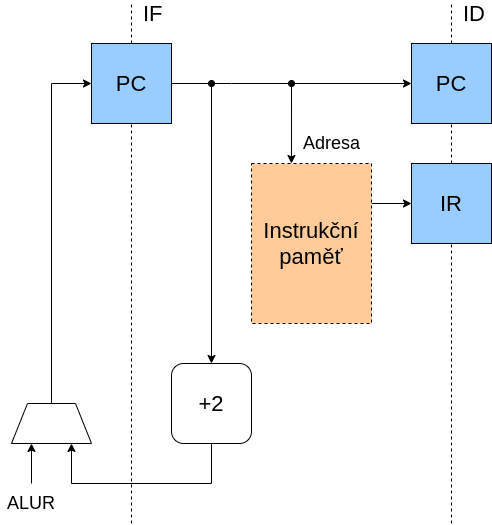
\includegraphics[height=0.3\textheight]{img/risc63-if}
  \end{center}
  \caption{Struktura fáze vyzvednutí instrukcí}
  \label{fig:if}
\end{figure}

IF fáze je prvním stupněm pipeline, kterým instrukce projde při svém zpracování uvnitř procesoru. IF fáze nastaví hodnotu adresy další instrukce do registru PC a následně adresuje instrukční paměť. Pokud nebyl indikován žádný typ skoku řadičem procesoru, pak následující instrukce bude vyzvednuta z adresy, jejíž hodnota je o dva vyšší. Instrukce totiž mají 16 bitů a očekávají paměť s adresací po bytech. Pokud byl indikován skok, bude použit výsledek ALU jako další hodnota PC, protože právě tam byla spočítána adresa další instrukce.

Obrázek \ref{fig:if} však vzhledem ke své jednoduchosti nepostihuje přerušení. Pokud by došlo k přerušení, do PC registru se zapíše hodnota \texttt{ivec}. V případe návratu z přeruše se použije hodnota \texttt{spc}.

Ačkoli registr PC má architekturální velikost 64 bitů, skutečná velikost PC je 63 bitů, protože nejnižší bit každé adresy instrukce je nula. V důsledku se pak nepřičítá hodnota dva, ale jedna. \newpage

\subsection{Fáze dekódování instrukce (ID)}
\begin{figure}[H]
  \begin{center}
    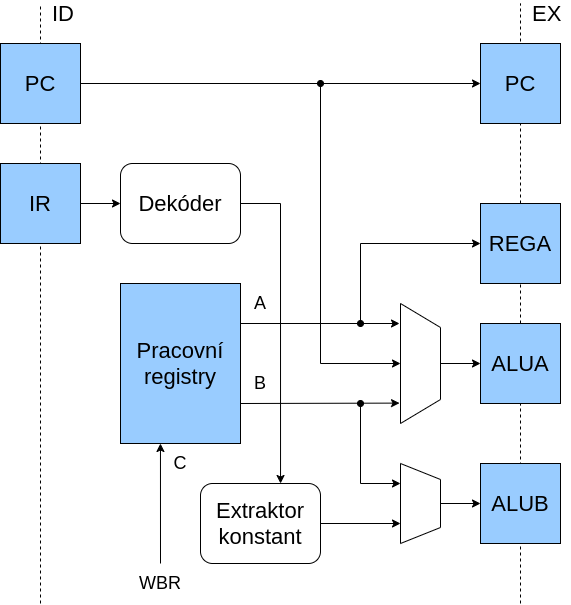
\includegraphics[height=0.3\textheight]{img/risc63-id}
  \end{center}
  \caption{Struktura fáze dekódování instrukcí}
\end{figure}

Po vyzvednutí instrukce z paměti je uložena v registru IR\footnote{Instruction Register -- instrukční registr}, odkud probíhá její další zpracování. Jsou z ní extrahovány indexy pracovních registrů, které jsou následovně přečteny. Vyšší byte instrukce je poslán do dekodéru, aby se určil formát instrukce a nastavily řídicí signály jako např. operační kód pro ALU. Na základě řídicích signálů extraktor konstant vybere zamýšlený rozsah bitů z instrukce jako konstantu a~znaménkově bity rozšíří na 64 bitů. Taktéž multiplexory obdrží řídicí signály a propagují dál požadované operandy pro ALU.

Dekódování instrukcí RISC63 architektury se ukazuje být docela komplikované. Vzhledem k typu ISA registr-registr a nejednotnosti konstant v instrukčním slově existuje mnoho výjimek, na které se musí brát zřetel v dekodéru. To vede ke zvýšení jeho složitosti.

V rámci této fáze probíhá i zápis do pracovních registrů z fáze WB jako výsledek některé z předcházejících instrukcí. Tento výsledek je okamžitě dostupný pro aktuálně dekódovanou instrukci. Mezi ID a WB je více fází pipeline, a tak výsledky libovolné předcházející instrukce dostupné být nemusí. Snaha použít nějaký takový výsledek vede k datovému hazardu (viz kapitola \ref{subsec:hazard}).

\subsection{Fáze provádění instrukce (EX)}
\begin{figure}[H]
  \begin{center}
    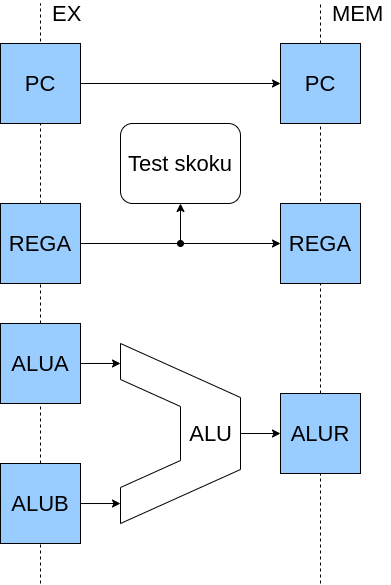
\includegraphics[height=0.3\textheight]{img/risc63-ex}
  \end{center}
  \caption{Struktura fáze provádění instrukcí}
\end{figure}

EX fáze provádí samotný výpočet požadovaný aktuální instrukcí v~ALU. Vstupem jsou jí dva operandy připravené z ID fáze. EX fáze zároveň určuje, zda se podmíněné skoky vykonají, nebo ne. K tomuto účelu byla doručena hodnota registru A ve speciálním registru, který je nezávislý na zvolených operandech ALU. Při skocích se totiž v ALU počítají výsledné adresy skoků a otestovat, zda se podmíněný skok provede, se musí jinde.

ALU jednotka implementuje v sobě dva moduly z důvodu dekompozice návrhu. Prvním modulem je 64bitová univerzální sčítačka. Na tuto jedinou sčítačku jsou mapovány všechny instrukce součtu, rozdílu i aritmetického porovnávání. Druhý modul umožňuje manipulaci s datovými bloky menšími než 64 bitů. Provádí extrakce, vkládání a~maskování. \newpage

\subsection{Fáze přístupu do paměti (MEM)}
\begin{figure}[H]
  \begin{center}
    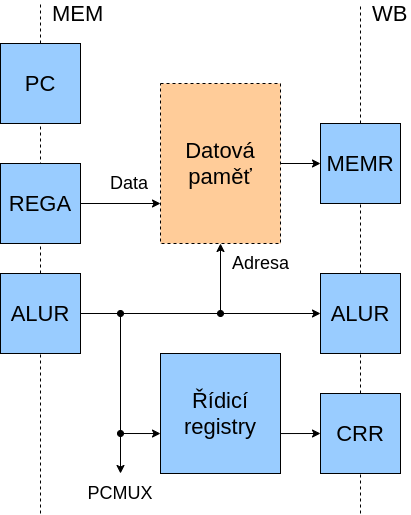
\includegraphics[height=0.3\textheight]{img/risc63-mem}
  \end{center}
  \caption{Struktura fáze přístupu do paměti}
\end{figure}

V MEM fázi může procesor komunikovat s datovou pamětí. Pro zápis používá registr A a jako adresu výsledek ALU. Obdobně jako pro cílové adresy skoků se v ALU počítají i cílové adresy dat. Z paměti lze číst výsledky všech předcházejících instrukcí bez rizika hazardu (viz kapitola \ref{subsec:interface}). Mimoto se v této fázi přistupuje i k řídícím registrům a~zápisy do nich mají také okamžitý efekt na následující instrukce.

MEM fáze také posílá signály související se skoky do řadiče procesoru. Pokud se jedná o obyčejné instrukce skoku, pak v registru výsledku ALU je již připravena adresa další instrukce. Pakliže jde o~instrukci návratu z přerušení, pochopitelně se použije hodnota \texttt{spc} registru, která je přímo vyvedena z řídících registrů.

Vzhledem k tomu, že se jedná o první fázi ovlivňující architekturální stav datového úložiště procesoru, má velmi důležitou roli i~pro přerušení. Pokud je totiž přerušení přijato, jsou veškeré zápisy této fáze zrušeny a PC hodnota registru této fáze je uložena do \texttt{spc}, odkud se pak bude pokračovat, protože žádný výsledek se nezapsal. Adresa další instrukce je hodnota registru \texttt{ivec}, která je taktéž vyvedená z řídících registrů. Vliv přerušení a skoků na pipeline je popsán v~kapitole~\ref{subsec:hazard}.

\subsection{Fáze zápisu výsledku (WB)}
\begin{figure}[H]
  \begin{center}
    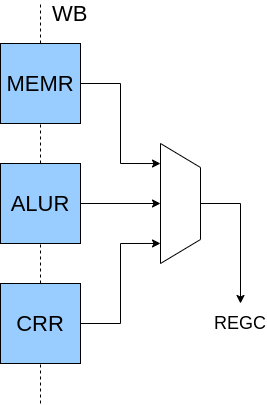
\includegraphics[height=0.3\textheight]{img/risc63-wb}
  \end{center}
  \caption{Struktura fáze zápisu výsledku}
\end{figure}

Fáze WB je poslední fází zpracování instrukce. Zapisuje výsledek do pracovního registru procesoru. Může to být přečtená hodnota z~paměti, ALU výsledek, nebo hodnota řídícího registru.

\subsection{Pipeline hazardy}
\label{subsec:hazard}
Zpracování instrukcí zřetězeným způsobem bývá doprovázeno negativním jevem označovaným jako hazard. Jedná se o stav procesoru, který může bezprostředně vést k chování procesoru, které neodpovídá sekvenční povaze vykonávaných instrukcí. Pro korektní chování procesoru za každých okolností se musí všechny možné hazardy identifikovat a ošetřit na úrovni hardware. Pokud mikroarchitektura trpí nějakým hazardem, lze k tomu přizpůsobit i software. Ten se pak musí vyhýbat kritickým situacím, které k iniciaci hazardu vedou. Nejedná se však o ideální řešení. Pro kontext této práce jsou důležité pouze dva typy hazardů -- řídící hazard a datový hazard.

Řídící hazard je úzce spojený se skoky a přerušením. V momentě, kdy se provádí v navrženém procesoru skok, vstup do rutiny přerušení nebo návrat z ní, řadič procesoru automaticky nastaví hodnotu reset signálu ID, EX a MEM fází jako aktivní na dobu jednoho hodinového signálu. To způsobí, že žádný výsledek jakékoliv již vyzvednuté instrukce po instrukci skoku nebude uložen. Mezitím IF fáze už vyzvedává instrukci z nové adresy PC registru a WB fáze dokončuje zápis instrukce před skokem. Oba tyto kontexty se pak bezkonfliktně potkají v ID fázi. Řídící hazardy jsou tedy ošetřené.

Datové hazardy momentálně ošetřeny nejsou, je potřeba se jim vyhnout softwarově. Pro vznik datového hazardů existuje jednoduché pravidlo. Pokud instrukce čte hodnotu registru, do kterého nějaká ze tří předcházejících instrukcí zapisovala, obdrží neaktuální hodnotu. A~to je datový hazard. Je způsoben skutečností, že se pracovní registry čtou ve fázi ID, kdežto výsledek se do nich zapisuje až ve fázi WB.

K řešení takových datových hazardů se obvykle používají dva přístupy. Buďto se zastaví část pipeline a počká se, až bude výsledek dostupný, nebo se výsledek propaguje zpátky z několika fází, nejen z~poslední. Čekání na výsledek při čtení paměti se ovšem reálně vyhnout nedá ani v tomto případě.

\section{Rozhraní pro komunikaci s pamětí}
\label{subsec:interface}
Procesor pro svůj korektní běh potřebuje instrukční a datovou paměť výhradně s asynchronním čtením. Datová paměť navíc musí podporovat synchronní zápis za použití stejného hodinového signálu jako procesor. Výsledná mikroarchitektura nepodporuje sdílení paměti, resp. zamítnutí požadavku přístupu k paměti, tudíž by mohly nastat problémy v případě potřeby přetvořit výslednou paměťovou hierarchii směřující k jedné společné operační paměti pro instrukce i data, čemuž architektura RISC63 jako taková nijak nebrání.

\subsection{Rozhraní pro instrukční paměť}
Procesor komunikuje s pamětí instrukcí za použití uvedených portů:

\begin{enumerate}
  \item Výstup 63bitový \texttt{o\_imem\_addr}\footnote{Pohybujeme se v 64bitovém adresním prostoru bytů a tento port adresuje paměť po slovech. Nejnižší bit tedy není nikdy potřeba.}
  \item Vstup 16bitový \texttt{i\_imem\_rd\_data}
\end{enumerate}

První uvedený port reprezentuje adresu a druhý přečtenou instrukci z této adresy. Čtení probíhá neustále.

\subsection{Rozhraní pro datovou paměť}
Komunikace s datovou pamětí používá následující porty:

\begin{enumerate}
  \item Výstup jednobitový \texttt{o\_dmem\_we}
  \item Výstup 61bitový \texttt{o\_dmem\_addr}\footnote{Bitová šířka je zvolena obdobně jako u \texttt{o\_imem\_addr} portu uvedeného dříve.}
  \item Výstup 64bitový \texttt{o\_dmem\_wr\_data}
  \item Výstup 64bitový \texttt{i\_dmem\_rd\_data}
\end{enumerate}

První uvedený port povoluje zápis do paměti. Druhý reprezentuje adresu paměti. Zbylé dva porty reprezentují zapisovaná a přečtená data. Čtení paměti probíhá neustále.

\section{Úvod do VHDL projektu}
\label{sec:project}
Vytvořený VHDL projekt, který je elektronickou přílohou této práce, dodržuje určité konvence a adresářovou strukturu. V této kapitole je podstatná část této problematiky vyjasněna.

\subsection{Použité konvence}
Každý datový objekt použitý ve zdrojových kódech projektu má ve svém identifikátoru předponu. Mimo datové objekty jsou předpony použity i pro identifikátory nějakých dalších konstrukcí VHDL. Tento přístup byl zaveden, protože na mnohá místa ve VHDL kódu lze použít více datových objektů. Následuje výčet použitých předpon:

\begin{itemize}
    \item \texttt{i\_} -- vstupní porty
    \item \texttt{o\_} -- výstupní porty
    \item \texttt{s\_} -- signály
    \item \texttt{v\_} -- proměnné
    \item \texttt{c\_} -- konstanty
    \item \texttt{t\_} -- vlastní datové typy
    \item \texttt{f\_} -- funkce
\end{itemize}

Uvedené předpony se neskládají a zanikají zároveň s asociovaným datovým objektem. Např. výstupní port \texttt{o\_cr\_ie} mapujeme na signál \texttt{s\_cr\_ie}, nikoli na \texttt{s\_o\_cr\_ie}. Pokud to jednoznačně nelze, zachováme i předponu. Snažíme se tomu však předejít.

Další adaptovanou konvencí v projektu je po této předponě uvést také předponu reprezentující komponentu, které této signál náleží (pokud nějaká existuje). Nejpoužívanějšími předponami jsou:

\begin{itemize}
    \item \texttt{cu\_} -- řadič procesoru
    \item \texttt{cr\_} -- řídící registry
    \item \texttt{if\_} -- IF fáze
    \item \texttt{id\_} -- ID fáze
    \item \texttt{ex\_} -- EX fáze
    \item \texttt{mem\_} -- MEM fáze
    \item \texttt{wb\_} -- WB fáze
\end{itemize}

\subsection{Adresářová struktura}
Projekt VHDL má následující adresářovou strukturu: \medskip

\dirtree{%
.1 risc63.
.2 rtl \DTcomment{VHDL popis mikroarchitektury}.
.3 if \DTcomment{vyzvednutí instrukce}.
.3 id \DTcomment{dekódování instrukce}.
.3 ex \DTcomment{provádění instrukce}.
.3 mem \DTcomment{přístup do paměti}.
.3 wb \DTcomment{zápis výsledku}.
.2 test \DTcomment{test bench moduly}.
.2 build \DTcomment{build systém, makefile}.
}

\chapter{Simulace mikroarchitektury}
Simulace mikroarchitektury je hlavním měřítkem korektnosti modelu navrženého procesoru ve VHDL.  K simulaci se používá program GHDL, který lze nainstalovat pomocí dostupných připravených binárních distribucí.\footnote{\url{https://github.com/ghdl/ghdl/releases}} Případně jej lze zkompilovat pro konkrétní systém podle návodu uvedeného v dokumentaci.\footnote{\url{https://ghdl.readthedocs.io/en/latest/getting/index.html}} Pro potřeby graficky zobrazit průběh přechodů signálů zvolené komponenty je používán program GTKWave\footnote{\url{http://gtkwave.sourceforge.net}}. Viz obrázek \ref{fig:gtkwave}.

\begin{figure}[H]
  \begin{center}
    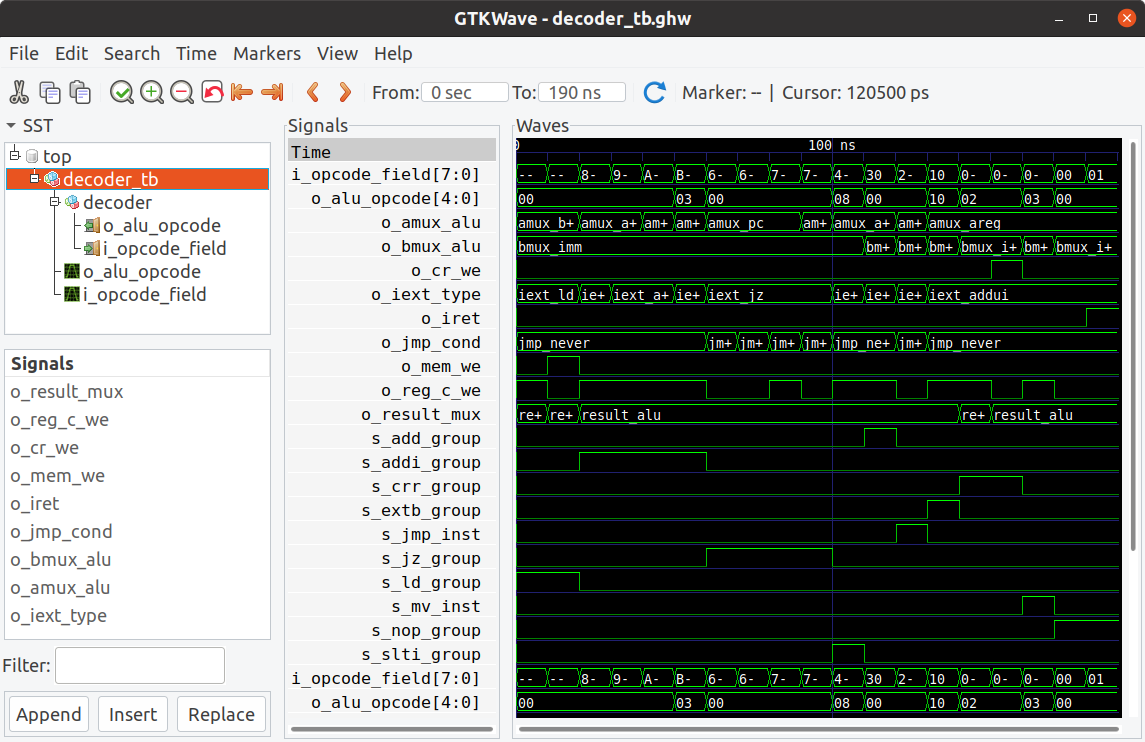
\includegraphics[height=0.4\textheight]{img/gtkwave}
  \end{center}
  \caption{Ukázka programu GTKWave}
  \label{fig:gtkwave}
\end{figure}

Samotná simulace a testování jsou pak prováděny prostřednictvím test bench souborů popsaných též v jazyce VHDL.\footnote{Určitá podmnožina jazyka VHDL je použitelná pouze pro simulační účely.} Test bench soubory provádí tzv. black-box testování. Vybere se VHDL komponenta a~obsáhne se v test bench modulu. Poté se řídí její vstupy a v závislosti na tom se kontrolují její výstupy vůči očekávaným výstupům.

\section{GHDL simulátor}
GHDL může být zkompilován tak, aby používal jeden z několika podporovaných back endů. V závislosti na back endu pak mohou existovat malé rozdíly v obsluze GHDL, avšak hlavní funkcionalita je se všemi back endy ekvivalentně dostupná.

Pro manuální spuštění testu pomocí GHDL je potřeba nejprve importovat všechny dotčené moduly (zahrnuje závislosti) do pracovní knihovny. Lze toho dosáhnout příkazem \texttt{ghdl -i <soubory>}. Poté je potřeba zkompilovat entitu testu. Toho lze dosáhnout příkazem \texttt{ghdl~-m~<entita>}. Tento příkaz zkompiluje i entity, které zadaná entita obsahuje. Pro samotné spuštění testu se pak používá příkaz \texttt{ghdl -r <entita>}.

\section{Vlastní build systém}
V průběhu vývoje RISC63 procesoru se ukázalo, že standardní API\footnote{Application Programming Interface -- rozhraní pro programování aplikací} programu GHDL nebude dostačovat pro další postup. Zejména bylo třeba automaticky kompilovat všechny entity a spustit všechny testy. Také byly požadovány možnosti zkompilovat jen jednu entitu a totéž se spuštěním testu. U spouštění testu pak volitelně spustit i náhled jeho průběhu v programu GTKWave. Každá taková funkce musela být dostupná prostřednictvím jednoho příkazu.

Jako řešení bylo zvoleno vytvoření POSIX\footnote{Portable Operating System Interface -- přenosné rozhraní pro operační systémy} \texttt{makefile} \parencite{ieee18}, který byl umístěn do adresáře \texttt{build}, kde také generuje pomocné soubory při vykonávání požadovaných úkonů. Tento soubor definuje několik cílů, které lze sestavit prostřednictvím \texttt{make} příkazu vyvolaného z adresáře \texttt{build}. Následuje seznam nejdůležitějších:

\begin{itemize}
    \item \texttt{elab} -- zkompiluje všechny entity
    \item \texttt{test} -- spustí testy všech test bench entit
    \item \texttt{elab\_a} -- zkompiluje entitu, jejíž název je uložen v makru \texttt{a}
    \item \texttt{test\_a} -- spustí test zadané entity
    \item \texttt{view\_a} -- spustí test zadané entity a zobrazí jeho průběh
    \item \texttt{clean} -- smaže všechny vygenerované soubory
\end{itemize}

V případě, že je do projektu přidán nový VHDL soubor, musí se aktualizovat i interní seznam projektových VHDL souborů uvedený v~\texttt{makefile}. Celý build systém byl otestován v Linuxovém prostředí (Ubuntu~18.04.4).

\chapter*{Závěr}
\addcontentsline{toc}{chapter}{Závěr}
Výsledkem práce je architektura vlastní instrukční sady, mikroarchitektura, která z ní vychází, a popis mikroarchitektury v jazyce VHDL včetně testů dokládajících její funkčnost. V průběhu práce byl stručně popsán celý proces vývoje modelu procesoru od počáteční definici pojmů přes volbu vlastností instrukční sady až po detailní popis práce pipeline cílené mikroarchitektury. Mnohá rozhodnutí jsou doložena odkazem na již existující procesorové architektury, protože mají klíčový vliv na tuto práci.

Volba instrukčního slova 16 bitů vedla k omezením při návrhu instrukční sady i při následné implementaci v mnohých ohledech. Několikrát bylo na tuto skutečnost poukázáno jako na negativní aspekt menších instrukcí. Práce tak naplnila původní motivaci prozkoumat dopady volby 16bitových instrukcí na návrh modelu procesoru a jeho architektury.

I navzdory obtížím při snaze implementovat mikroarchitekturu efektivně, se podařilo navrhnout a zrealizovat přerušovací systém procesoru. Způsob fungovaní přerušení je velmi jednoduchý a přitom důmyslný. Přerušení jsou navíc akceptována okamžitě, což nebývá pravidlem při použití pipeline.

Klíčová vlastnost, která procesoru chybí, je schopnost se vypořádat s datovými hazardy v pipeline. V práci byly zmíněny dvě možné metody řešení tohoto problému a lze to považovat za směr budoucího vývoje RISC63 procesoru. Eliminací datových hazardů se totiž sníží velikost aktuálních programů a RISC63 bude moci dostát svému původnímu záměru.

\printbibliography[heading=bibintoc] %% Print the bibliography.
\appendix %% Start the appendices.
\chapter{Elektronické přílohy}
Jedinou elektronickou přílohou práce je implementace popsané mikroarchitektury. Krátký úvod k implementaci je uveden v kapitole \ref{sec:project}.

\chapter{Schéma pipeline}
\label{app:pipeline}
\begin{figure}[H]
  \begin{center}
    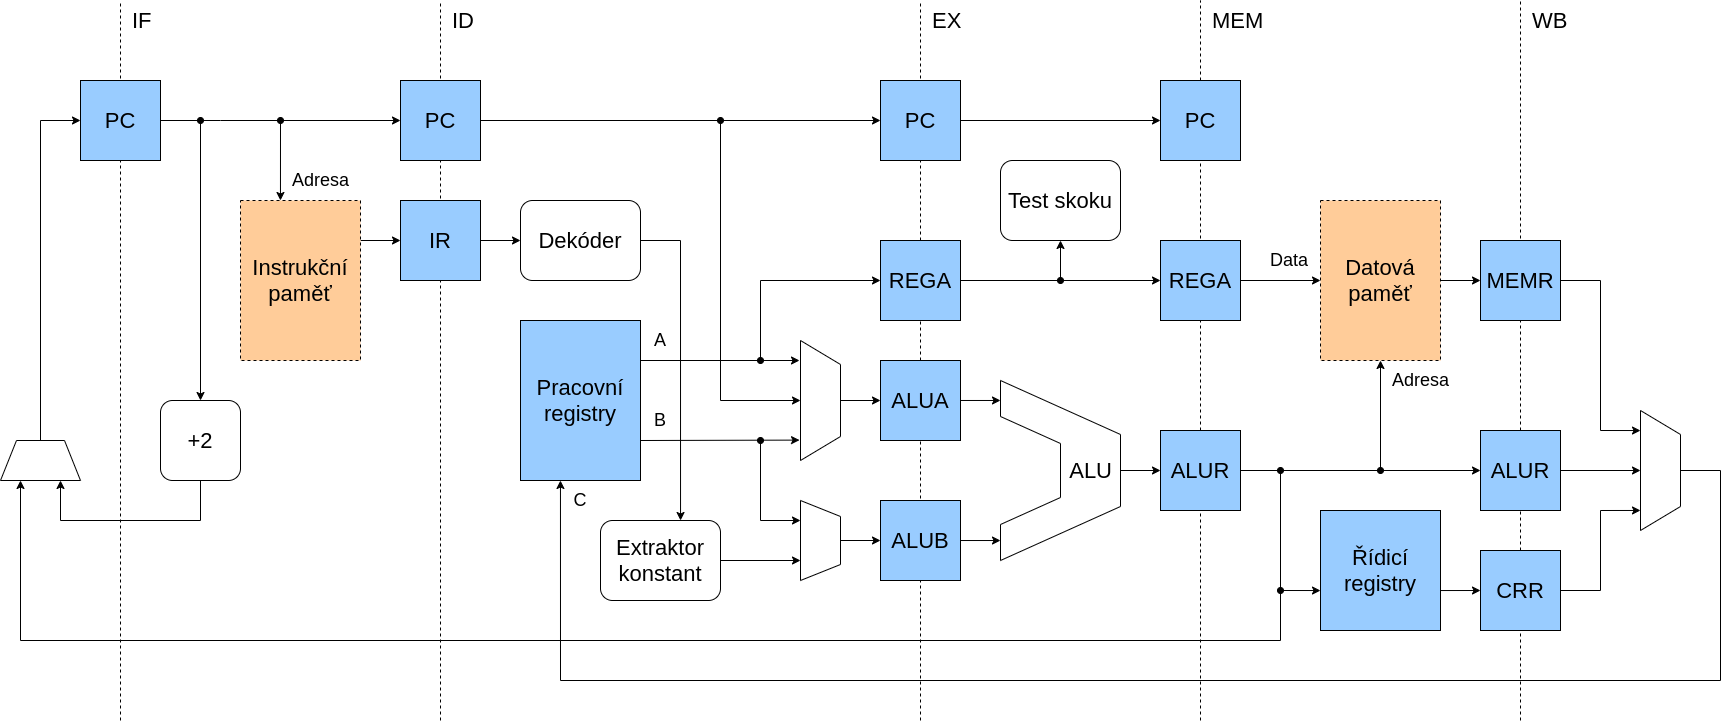
\includegraphics[height=0.5\textwidth, angle=-90]{img/risc63-pipeline}
  \end{center}
  \caption{Struktura pipeline implementované mikroarchitektury}
\end{figure}
\end{document}
